%%%%%%%%%%%%%%%%%%%%%%%%%%%%%%%%%%%%%%%%%%%%%%%%%%%%%%%%%%%%%%%%%%%%%%%%%%%%%%%%
\newpage\section{Orbit Determination and Parameter Estimation}
%%%%%%%%%%%%%%%%%%%%%%%%%%%%%%%%%%%%%%%%%%%%%%%%%%%%%%%%%%%%%%%%%%%%%%%%%%%%%%%%

Predicting the state ($\bm{x}_t$) of a spacecraft given an initial condition
($\bm{x}_0$), and models which form the equations of motion of the satellite,
($\dot{\bm{x}}=f(t,\bm{x})$), is a straightforward task involving the solution
of an initial value problem (IVP) in the form of an ordinary differential
equation (ODE). However the inverse problem  is more involved, that is, given a
set of measurements ($\bm{z}$) resulting from the dynamical system, we would
like to estimate the trajectory of the satellite and the parameters describing
the dynamical models, described mathematically as:
\begin{equation}
    \bm{x}(t) =
    \begin{bmatrix}
        \bm{r}(t) \\
        \bm{v}(t) \\
        \bm{p} \\
        \bm{q} \\
    \end{bmatrix}.
\end{equation}
\begin{equation*}
    \begin{aligned}
        \textrm{where  }
            \bm{r}(t), \bm{v}(t) &= \text{the position and velocity of the spacecraft as a function of time,} \\
            \bm{p}               &= \text{the parameters describing the force models,} \\
            \bm{q}               &= \text{the parameters describing the measurement models.} \\
    \end{aligned}
\end{equation*}

The measurements made throughout the trajectory of the spacecraft at times
$t_1,...,t_n$ are described by $\bm{z}=[z_1,...,z_n]$, where each $z_i$ is
either defined as a function of the state of the spacecraft at time $t_i$, or
as a function of the state of the spacecraft at time $t_0$:
\begin{equation}
    z_i(t_i) = g_i(t_i, \bm{x}(t_i))+\epsilon_i = h_i(t_i, \bm{x}_0)+\epsilon_i
\end{equation}
\begin{equation*}
    \begin{aligned}
        \textrm{where  }
            z_i &= \text{the i$^{th}$ empirical measurement, assumed to be a random variable,} \\
            g_i &= \text{the i$^{th}$ modelled measurement as a function time and instantaneous state,} \\
            h_i &= \text{the i$^{th}$ modelled measurement as a function time and initial state,} \\
            \epsilon_i &= \text{the i$^{th}$ residual, accounting for measurement errors.} \\
    \end{aligned}
\end{equation*}

The expressions of $h_i$ and $g_i$ can be used interchangeably in the
measurement model predictions, to account for the fact that the measurements
are often made at different times than their respective instantaneous states of
the spacecraft. This is done through the use of variational equations, which
are simulated to obtain the state transition matrix $\bm{\Phi}(t_0, t_j)$ of the
spacecraft, as described in \autoref{sec:linearization}, which may be
interpolated for any arbitrary time within the temporal bounds of the ODE
solution across $t_i\in\[t_0, t_f]$.





%\begin{figure}[h]
%    \centering
%    \def\svgwidth{0.95\linewidth}
%    % \input{graphics/drawing2.pdf_tex}
%    \import{graphics/}{trajectory_estimation.pdf_tex}
%    \caption{Definition of a general Body-centered inertial (BCI) reference frame.}
%    \label{fig:as}
%\end{figure}


%Furthermore, the accuracy of this solution can be
%traded off against the computational expense of the prediction.

%
%\begin{itemize}
%    \item Orbit of asteroid
%    \item Orbit of spacecraft
%    \item Rotation of asteroid (rate + principle axes)
%    \item Gravitational potential of asteroid
%\end{itemize}




\begin{equation}
    z = \mathbf{h}(\mathbf{x}_0) + \mathbf{\epsilon}
\end{equation}

%%%%%%%%%%%%%%%%%%%%%%%%%%%%%%%%%%%%%%%%%%%%%%%%%%%%%%%%%%%%%%%%%%%%%%%%%%%%%%%%
\newpage\subsubsection{Weighted Least-Squares Estimation}
%%%%%%%%%%%%%%%%%%%%%%%%%%%%%%%%%%%%%%%%%%%%%%%%%%%%%%%%%%%%%%%%%%%%%%%%%%%%%%%%

The Weighted Least-Squares Estimation method is an application of the
Generalized Least-Squares (GLS) algorithm~\cite{Aitken1936}, which aims at
estimating unknown parameters ($\bm{x}$) in a linear regression model, given a
set of observations ($\bm{y}$), where there is a certain degree of correlation
($\bm{W}$) between the residuals ($\bm{\epsilon}$) in the regression model:
\begin{equation}
\bm{y}=\bm{A}\bm{x}+\bm{\epsilon},\;\;\;\gls{E}{}[\bm{\epsilon}]=\bm{0},\;\;\;\text{Cov}(\bm{\epsilon}|
\bm{A})=\bm{W}. \label{eq:linear-regression} \end{equation}

The problem arises when considering the non-linear dynamics experienced by the
spacecraft throughout its trajectory, which is not entirely described by
\autoref{eq:linear-regression}. The


\begin{equation}
    H=\frac{\partial{\bm{h}(x_0)}}{\partial{\bm{x}_0}}\bigg|_{\mathbf{x}_0}
\end{equation}

\begin{equation}
    \Delta{\bm{q}}=K(H^{T}W\Delta{\bm{h}})
\end{equation}

\begin{equation}
    K=(H^{T}WH)^{-1}
\end{equation}

\subsubsection{Linearization \& Normal Equations}

\subsubsection{Filtering}


 \noindent{}A CEKF consists of 3 main steps, namely: \textit{Initialisation (0)}, \textit{Prediction (1)} and \textit{Correction (2)}, where steps 1 \& 2 are iterated through $K-1$ times, where $K$ ($K\in\mathbb{Z}^+$) quantifies the number of Epochs.

 \begin{itemize}
     \item \textbf{Step (0) Initialisation}: The \textit{a posteriori} estimate of the initial state ($\hat{x}_0^+$) is determined according to the expectation of the true value $x_0$. The initial state error co-variance matrix is calculated according to the expectation of the co-variance between $\hat{x}_0^+$ and $x_0$. Within the context of satellite tracking, a predefined $\hat{x}_0^+$ will be used throughout the CEKF analysis to analyse the performance as a result of the selection of hyper-parameters: $\bm{Q}_{k-1}$ and $\bm{R}_k$.
     \item \textbf{Step (1) Prediction}: Project the state and its co-variance matrix at $k-1$ one step forward in order to obtain the \textit{a priori} estimates at $k$ according to the system dynamics. $\bm{Q}_{k-1}$ is implemented, then this contributes to the \textit{a priori} estimate of $P_k^{}$.
    \item \textbf{Step (2) Correction}: The measurements at $k$ are then compared with the predicted state according to system dynamics (\textit{a priori} estimate) providing the \textit{measurement innovation} ($\Delta{\rho}_k$). \textit{innovation co-variance} ($S_k$) and $H_k$ are then calculated and used to obtain the \textit{Kalman gain} ($\overline{K}_k$). Finally the \textit{a posteriori} estimate of the state ($\hat{x}_k^+$) and co-variance ($P_k^+$) are determined. $k$ is incremented by a step forward and the process from step 1 is repeated for all Epochs.
 \end{itemize}

\begin{figure}[htp]
    \centering
    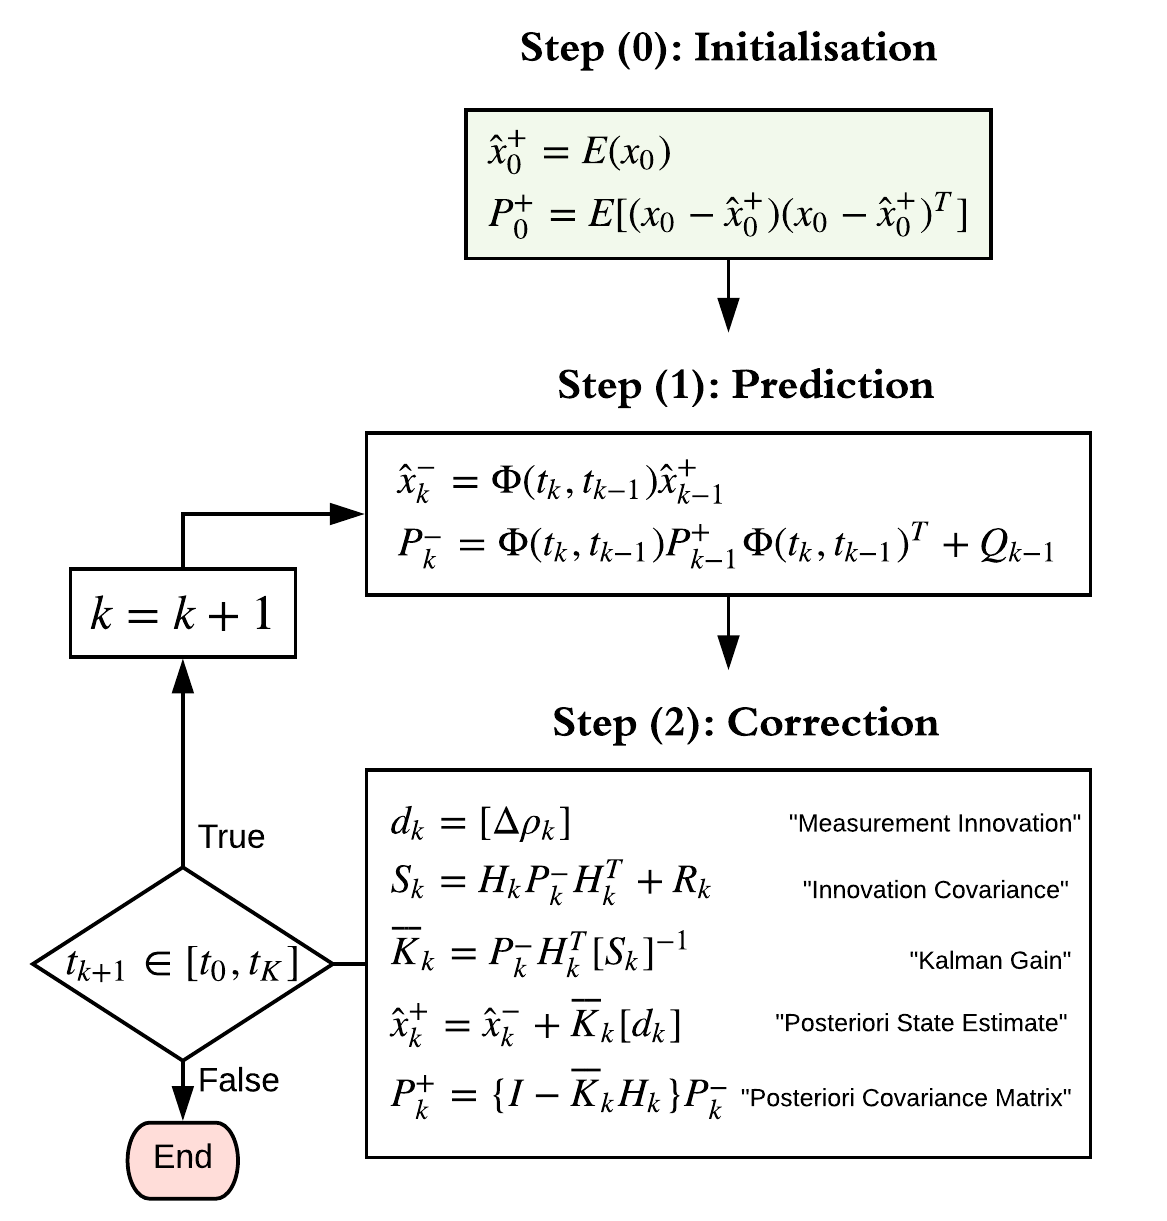
\includegraphics[width=0.55\linewidth]{graphics/CEKF.png}
    \caption{CEKF flow diagram for process of tracking and data prediction including all equations \cite{3}.}
    \label{fig:CEKF}
\end{figure}


\begin{figure}[htp]
    \centering
    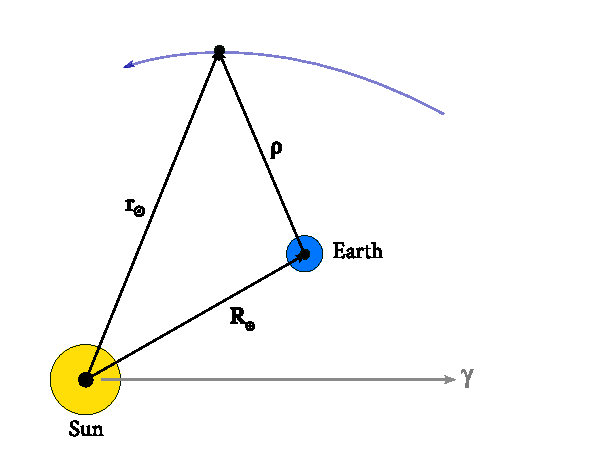
\includegraphics[width=0.5\linewidth]{graphics/pod-1.pdf}
    \caption{Orbit determination of asteroid using range observations from Earth ($\rho$).}
    \label{fig:my_label}
\end{figure}
